
% ------------------------------------------------------------------------
% ------------------------------------------------------------------------
% MODELO DE RELATÓRIO PARA BOLSA DO PROJETO SISRAS2
% Baseado no Abntex2
% Por Chrystian de Sousa Guth (csguth <at> gmail <dot> com)
% ------------------------------------------------------------------------ 
% ------------------------------------------------------------------------

\documentclass[
	% -- opções da classe memoir --
	12pt,				% tamanho da fonte
	openright,			% capítulos começam em pág ímpar (insere página vazia caso preciso)
	twoside,			% para impressão em verso e anverso. Oposto a oneside
	a4paper,			% tamanho do papel. 
	% -- opções da classe abntex2 --
	%chapter=TITLE,		% títulos de capítulos convertidos em letras maiúsculas
	%section=TITLE,		% títulos de seções convertidos em letras maiúsculas
	%subsection=TITLE,	% títulos de subseções convertidos em letras maiúsculas
	%subsubsection=TITLE,% títulos de subsubseções convertidos em letras maiúsculas
	% -- opções do pacote babel --
	english,			% idioma adicional para hifenização
	french,				% idioma adicional para hifenização
	spanish,			% idioma adicional para hifenização
	brazil,				% o último idioma é o principal do documento
	]{abntex2}

% ---
% PACOTES
% ---

% ---
% Pacotes fundamentais 
% ---
\usepackage{lmodern}			% Usa a fonte Latin Modern
\usepackage[T1]{fontenc}		% Selecao de codigos de fonte.
\usepackage[utf8]{inputenc}		% Codificacao do documento (conversão automática dos acentos)
\usepackage{indentfirst}		% Indenta o primeiro parágrafo de cada seção.
\usepackage{color}				% Controle das cores
\usepackage{graphicx}			% Inclusão de gráficos
\usepackage{microtype} 			% para melhorias de justificação
\usepackage{listings}			% para inserir listagens
% ---

% ---
% Pacotes adicionais, usados apenas no âmbito do Modelo Canônico do abnteX2
% ---
\usepackage{lipsum}				% para geração de dummy text
% ---

% ---
% Pacotes de citações
% ---
\usepackage[brazilian,hyperpageref]{backref}	 % Paginas com as citações na bibl
\usepackage[alf]{abntex2cite}	% Citações padrão ABNT

% ---
% Customizacoes
% ---
\usepackage{sisras2}

% --- 
% CONFIGURAÇÕES DE PACOTES
% --- 

% ---
% Configurações do pacote backref
% Usado sem a opção hyperpageref de backref
\renewcommand{\backrefpagesname}{Citado na(s) página(s):~}
% Texto padrão antes do número das páginas
\renewcommand{\backref}{}
% Define os textos da citação
\renewcommand*{\backrefalt}[4]{
	\ifcase #1 %
		Nenhuma citação no texto.%
	\or
		Citado na página #2.%
	\else
		Citado #1 vezes nas páginas #2.%
	\fi}%
% ---

% ---
% Informações de dados para CAPA e FOLHA DE ROSTO
% ---
\titulo{Relatório de Atividades de Bolsista SisRas2\\(Junho de 2013 a Janeiro de 2014)}
\autor{Chrystian de Sousa Guth}
\local{Florianópolis}
\data{Janeiro de 2014}
\instituicao{Universidade Federal de Santa Catarina}
\tipotrabalho{Tese (Doutorado)}
% O preambulo deve conter o tipo do trabalho, o objetivo, 
% o nome da instituição e a área de concentração 
\preambulo{}
% ---

% ---
% Configurações de aparência do PDF final

% alterando o aspecto da cor azul
\definecolor{blue}{RGB}{41,5,195}

% informações do PDF
\makeatletter
\hypersetup{
     	%pagebackref=true,
		pdftitle={\@title}, 
		pdfauthor={\@author},
    	pdfsubject={\imprimirpreambulo},
	    pdfcreator={LaTeX with abnTeX2},
		pdfkeywords={abnt}{latex}{abntex}{abntex2}{projeto de pesquisa}, 
		colorlinks=true,       		% false: boxed links; true: colored links
    	linkcolor=blue,          	% color of internal links
    	citecolor=blue,        		% color of links to bibliography
    	filecolor=magenta,      		% color of file links
		urlcolor=blue,
		bookmarksdepth=4
}
\makeatother
% --- 

% --- 
% Espaçamentos entre linhas e parágrafos 
% --- 

% O tamanho do parágrafo é dado por:
\setlength{\parindent}{1.3cm}

% Controle do espaçamento entre um parágrafo e outro:
\setlength{\parskip}{0.2cm}  % tente também \onelineskip

% ---
% compila o indice
% ---
\makeindex
% ---

% ----
% Início do documento
% ----
\begin{document}

% Retira espaço extra obsoleto entre as frases.
\frenchspacing 

% ----------------------------------------------------------
% ELEMENTOS PRÉ-TEXTUAIS
% ----------------------------------------------------------
% \pretextual

% ---
% Capa
% ---
\imprimircapa
% ---

% ---
% Folha de rosto
% ---
%\imprimirfolhaderosto
% ---

% ---
% NOTA DA ABNT NBR 15287:2011, p. 4:
%  ``Se exigido pela entidade, apresentar os dados curriculares do autor em
%     folha ou página distinta após a folha de rosto.''
% ---

% ---
% inserir lista de ilustrações
% ---
%\pdfbookmark[0]{\listfigurename}{lof}
%\listoffigures*
%\cleardoublepage
% ---

% ---
% inserir lista de tabelas
% ---
%\pdfbookmark[0]{\listtablename}{lot}
%\listoftables*
%\cleardoublepage
% ---

% ---
% inserir lista de abreviaturas e siglas
% ---
%\begin{siglas}
%  \item[ABNT] Associação Brasileira de Normas Técnicas
%  \item[abnTeX] ABsurdas Normas para TeX
%\end{siglas}
% ---

% ---
% inserir lista de símbolos
% ---
%\begin{simbolos}
%  \item[$ \Gamma $] Letra grega Gama
%  \item[$ \Lambda $] Lambda
%  \item[$ \zeta $] Letra grega minúscula zeta
%  \item[$ \in $] Pertence
%\end{simbolos}
% ---

% ---
% inserir o sumario
% ---
%\pdfbookmark[0]{\contentsname}{toc}
%\tableofcontents*
%\cleardoublepage
% ---


% ----------------------------------------------------------
% ELEMENTOS TEXTUAIS
% ----------------------------------------------------------
\textual


\chapter{Relatório de Atividades do Bolsista}
% ----------------------------------------------------------
% Identificação
% ----------------------------------------------------------
\section{Identificação}

\begin{itemize}
	\item \textbf{Nome:} Chrystian de Sousa Guth;
	\item \textbf{Local de Trabalho:} Universidade Federal de Santa Catarina;
	\item \textbf{Título do Plano de Trabalho:} Avaliação do Impacto do Atraso das Interconexões na Análise de \textit{Timing} no Contexto de uma Ferramenta de \textit{Gate Sizing};
	\item \textbf{Tipo de Bolsa:} ITI-A;
	\item \textbf{Número do Processo da Bolsa:} 182980/2013-8;
	\item \textbf{Período:} Julho de 2013 - Janeiro de 2014;
	\item \textbf{Orientador:} José Luís Almada Güntzel (INE/UFSC);
	\item \textbf{Coordenador do Projeto:} Ricardo Augusto da Luz Reis (II/UFRGS).
\end{itemize}

% ----------------------------------------------------------
% Resumo 
% ----------------------------------------------------------
\section{Resumo}
Este documento relata as atividades realizadas pelo bolsista Chrystian de Sousa Guth no período de Junho de 2013 a Janeiro de 2014, no contexto de bolsa ITI-A associada ao ``Projeto SisRAS2 - Sistemas Computacionais com Capacidade de Confiabilidade, Disponibilidade e Utilidade (RAS) 2''.

Conforme previsto no plano de trabalho da bolsa, entre Junho de 2013 e Janeiro de 2014 o bolsista realizou um estudo para compreensão das técnicas de análise de \textit{timing} estática (\textit{STA: Static Timing Analysis}) aplicadas no contexto de uma ferramenta de otimização para fluxo industrial.

Nos primeiros meses (entre Junho e Setembro de 2013), o aluno desenvolveu uma ferramenta de STA utilizando a infraestrutura disponibilizada pela competição de \textit{sizing} discreto do ISPD 2013 \cite{Contest2013}, que levava em consideração o atraso das interconexões e a degradação do \textit{slew} através destas. Posteriormente, entre Outubro e Novembro de 2013, foram realizados experimentos a fim de validar a ferramenta, a qual foi documentada na forma de uma monografia de conclusão de curso, apresentada no presente trabalho na Seção \ref{sec:tcc}. Finalmente, entre Dezembro de 2013 e Janeiro de 2014, a infraestrutura implementada até então começou a ser incorporada à uma técnica de otimização para fluxo \textit{Standard Cell} conhecida como \textit{gate sizing}.

\begin{center}
\textit{\textbf{Palavras-chave:} automação de projeto eletrônico, biblioteca standard cell, análise de timing estática, complementary metal-oxide semiconductor, gate sizing.}
\end{center}

\section{Introdução}
O crescimento da complexidade dos circuitos digitais contemporâneos\footnote{Um processador para \textit{desktop} desenvolvido no ano de 2008 tem cerca de 731 milhões de transistores, excluindo a área de memória \cite{Intel08}.} e a necessidade de um \textit{time-to-market} (tempo de entrega ao mercado) curto faz com que o projeto de tais circuitos adote o fluxo \textit{standard cell}.

Os projetos de circuitos digitais no fluxo \textit{standard cell} são realizados visando, além das funcionalidades requisitadas, a operação em uma frequência especificada. Por isso, diversas otimizações são efetuadas ao longo do fluxo, para que tais funcionalidades consigam ser realizadas na frequência definida.

Análise de \textit{timing} estática, ou \textit{static timing analysis} \cite{Guntzel00} \cite{BhaskerChadha09}, é uma das técnicas utilizadas para se estimar o atraso crítico de circuitos digitais. A análise de \textit{timing} é chamada de estática quando ela não realiza simulação e portanto, independe de estímulos de entrada, considerando apenas a topologia do circuito. É um processo completo e exaustivo \cite{BhaskerChadha09} que verifica as mais diversas informações de \textit{timing} em um circuito, como os \textit{delays}, \textit{slews}, \textit{slacks} (folgas), \textit{required times} (tempos requeridos) e diversas violações de restrições de projeto.

Uma ferramenta capaz de realizar a análise de \textit{timing}, considerando os atrasos das interconexões, foi desenvolvida, implementando um modelo de grafo otimizado, obtendo tempos de execução cerca de 17 vezes menor que os tempos gastos em uma ferramenta industrial.


\section{Materiais e Métodos}

Nas atividades realizadas foi disponibilizado para uso do bolsista um computador tipo PC com sistema operacional Linux e outros recursos disponíveis no Laboratório de Computação Embarcada (ECL) da UFSC \cite{ECL}, como impressora \textit{laser}, rede de dados etc. Além dos recursos materiais, também foi utilizada a ferramenta de EDA (\textit{Electronic Design Automation}) Synopsys \textregistered \textit{PrimeTime} \texttrademark \cite{PrimeTime12}, para validação da técnica de STA implementada.

\section{Revisão Bibliográfica}

Com o objetivo de avaliar uma técnica para cálculo das características temporais das interconexões na análise de \textit{timing}, o bolsista realizou uma pesquisa em algumas técnicas e nos manuais do \textit{PrimeTime}. 

A técnica para cálculo do atraso das características temporais das interconexões implementada é baseada no trabalho \cite{PURI02} que por sua vez, ataca as principais desvantagens de se utilizar a abordagem apresentada em \cite{Kashyap00}.

\section{Experimentos Desenvolvidos, Resultados e Discussões}

\subsection{Definição do Modelo de Grafo do Circuito}
Para que a análise de \textit{timing} seja realizada, é necessário primeiramente, definir um modelo de grafo para representar o circuito. O modelo de grafo escolhido representa os \textit{Timing Points} no conjunto de vértices e os \textit{Timing Arcs} e interconexões no conjunto das arestas (Figura \ref{fig:grafo_timing_points}). Também são criados vértices especiais, chamados \textit{fonte} e \textit{terminal}. Estes nodos são inseridos no início e no fim do grafo, para que o mesmo possua apenas um ponto de ``entrada'', e um ponto de ``saída''.

\begin{figure}[ht]
\begin{center}
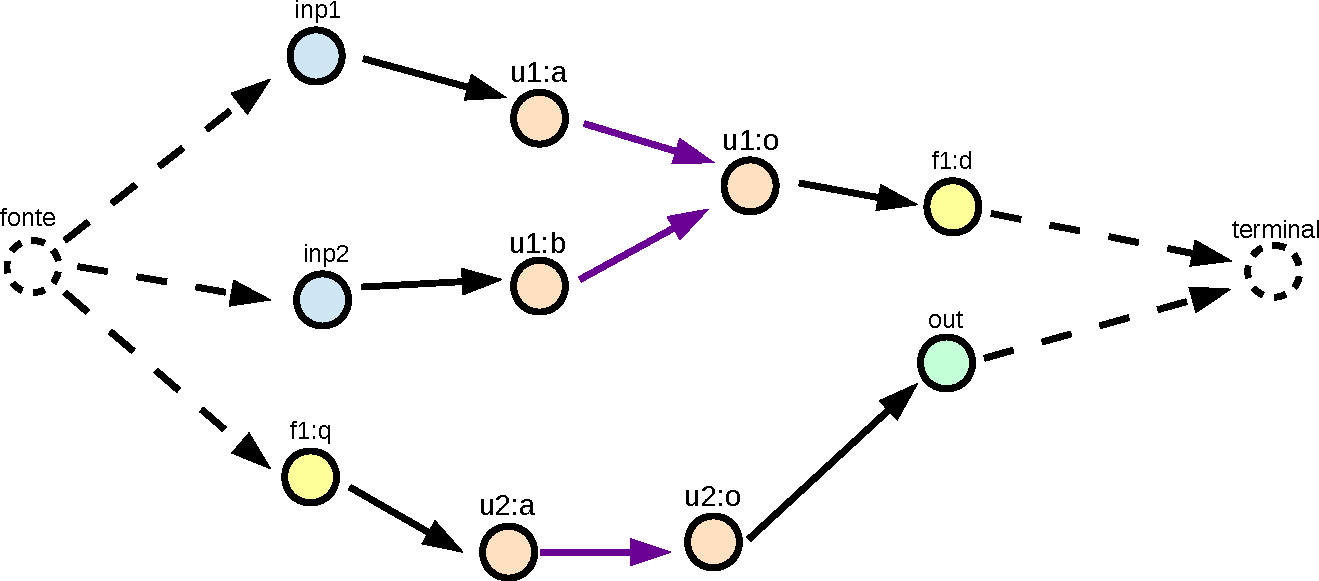
\includegraphics[width=\linewidth]{img/grafo_timing_points.pdf} 
\caption{Grafo de \textit{timing} com representação dos \textit{timing points}, \textit{timing arcs} e interconexões.}
\label{fig:grafo_timing_points}
\end{center}
\end{figure}



\subsection{Representação das Interconexões}
As interconexões mais complexas devem ser representadas levando em consideração suas características resistivas e capacitivas. Essas então, são modeladas como árvores RC (Figura \ref{fig:rc}), que conforme \citeonline{Rabaey08}, têm as seguintes características: 

\begin{itemize}
\item A rede tem apenas um nodo de entrada, chamado de \textbf{fonte} (\textit{source});
\item Todos os capacitores são entre um nodo e o terra;
\item A rede não possui \textit{loops} resistivos, por isso é chamada de Árvore.
\end{itemize}

\begin{figure}[ht]
\begin{center}
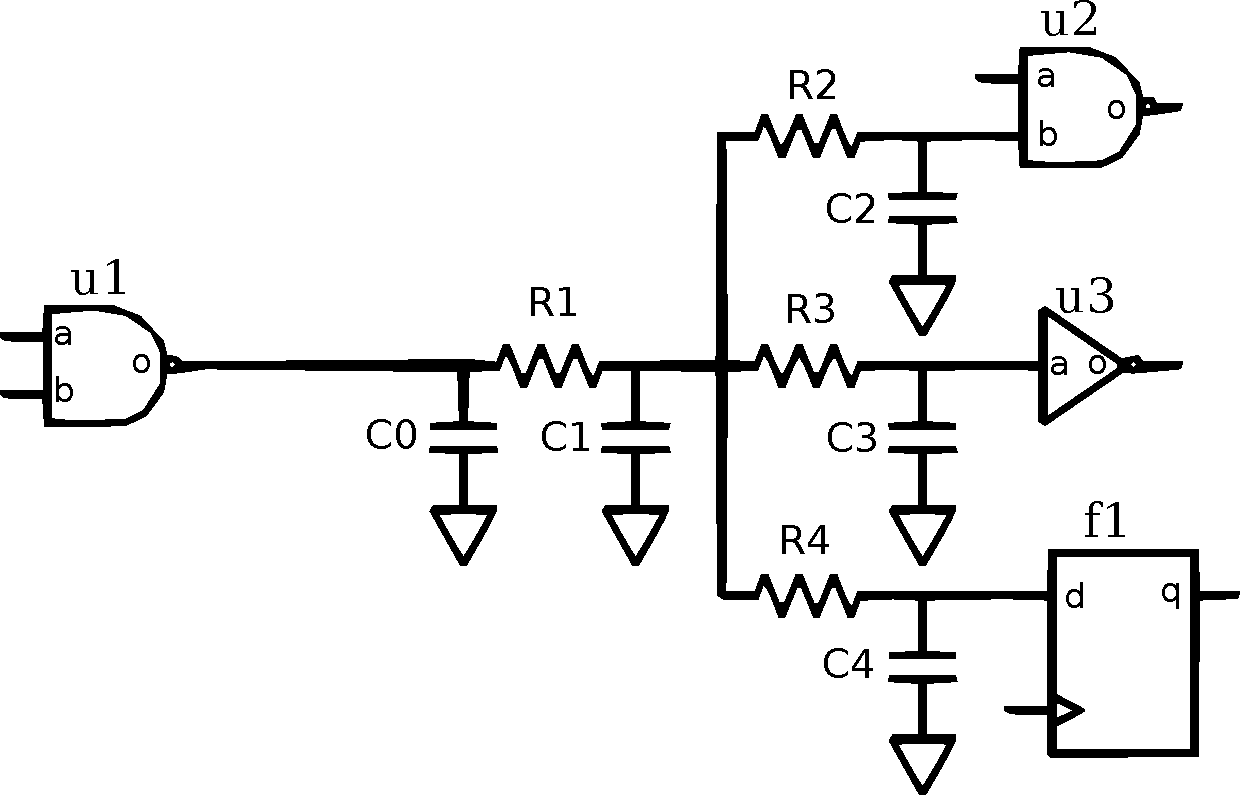
\includegraphics[width=0.7 \linewidth]{img/rc.pdf} 
\caption{Um circuito composto por três portas lógicas (\textit{u1, u2 e u3}), uma célula sequencial (\textit{f1}) e uma interconexão em forma de árvore RC, que liga a saída de \textit{u1} às entradas de \textit{u2, u3 e f1}. A interconexão em questão possui 5 capacitores (\textit{C0 (fonte), C1, C2, C3 e C4}) e 4 resistores (\textit{R1, R2, R3 e R4}).}
\label{fig:rc}
\end{center}
\end{figure}

\subsection{Algoritmo para o Cálculo das Informações Temporais das Interconexões}

\citeonline{Kashyap00} propuseram uma técnica para calcular o atraso da interconexão levando em conta o efeito de \textit{resistive shielding}. Com a mesma complexidade da técnica de Elmore, a técnica proposta para cálculo de atraso em uma árvore RC calcula também o valor de capacitância efetiva. Porém, \citeonline{Kashyap00} não consideravam o \textit{driver} da interconexão como sendo uma porta lógica \textit{CMOS}. Como consequência, sua aproximação para o \textit{slew} na entrada da árvore RC era imprecisa. Como o cálculo da capacitância efetiva de uma árvore depende do \textit{slew} que incide nesta, e o \textit{slew} depende da capacitância vista pelo \textit{driver}, \citeonline{PURI02} propuseram uma técnica que leva em consideração o impacto da capacitância no \textit{slew} do driver, e também, do \textit{slew} no cálculo da capacitância efetiva. Esta técnica foi implementada na ferramenta desenvolvida, e foi validada frente a uma ferramenta industrial.

\subsection{Cálculo do Atraso das Portas Lógicas}
Nas bibliotecas \textit{standard cell} atuais, modelos de atrasos não-lineares\footnote{Conhecidos na indústria por \textit{NLDM} (\textit{Non-Linear Delay Model})} são fornecidos para os \textit{timing arcs} das células disponíveis. Esses modelos, que geralmente são obtidos através de simulações em nível elétrico, são armazenados na forma de \textit{lookup tables}, como a da Figura \ref{fig:lookup_table}. Uma \textit{lookup table} descreve o \textit{delay} ou o \textit{slew} de uma célula em função de dois fatores: o \textit{slew} na entrada do \textit{timing arc} (colunas), e a capacitância de saída (\textit{load}) (linhas).

Utilizando a \textit{lookup table} da Figura \ref{fig:lookup_table} para estimar o \textit{delay} de um dos \textit{timing arcs} de uma célula \textit{CMOS} e supondo que o \textit{slew} na entrada deste \textit{timing arc} seja de $8.0$, e a capacitância vista na saída seja $0.1$, obtém-se que $delay = 3.49$, pois $3.49$ é o valor endereçado pelos índices da função (\textit{slew} e \textit{load}). Caso os valores de \textit{slew} ou \textit{load} não existam na tabela, uma interpolação linear é realizada. Da mesma forma, o cálculo do \textit{slew} do \textit{timing arc} é realizado com base na \textit{lookup table} específica para o \textit{slew}.

\begin{figure}[ht]
\lstset{basicstyle=\footnotesize}
\begin{lstlisting}[frame=single]
rise_delay (delay_table) {
 load (0.0, 0.1, 0.2, 0.4, 0.8, 1.6, 3.2) ;
 input_slew (0.5, 3.0, 5.0, 8.0, 14.0, 20.0, 30.0, 50.0) ;
 values (
   1.17, 1.82, 2.26, 2.76, 3.48, 4.04, 4.82, 6.12,
   1.69, 2.34, 2.86, 3.49, 4.41, 5.11, 6.06, 7.58,
   2.21, 2.86, 3.38, 4.12, 5.22, 6.05, 7.16, 8.90,
   3.25, 3.90, 4.42, 5.20, 6.60, 7.67, 9.08, 11.23,
   5.33, 5.98, 6.50, 7.28, 8.84, 10.30, 12.24, 15.14,
   9.50, 10.15, 10.67, 11.45, 13.01, 14.57, 17.15, 21.33,
   17.83, 18.48, 19.00, 19.78, 21.34, 22.90, 25.50, 30.70
  );
}
\end{lstlisting}
\caption{Uma \textit{lookup table} para atraso de subida (\textit{rise delay}) de um arco de \textit{timing}. As linhas são endereçadas por \textit{load} (capacitância de saída da porta lógica) e as colunas por \textit{input slew} (\textit{slew} aplicado na entrada do \textit{timing arc}). Adaptada de \cite{Contest2013}.}
\label{fig:lookup_table}
\end{figure}



\subsection{Algoritmo para o Cálculo do Atraso do Circuito (Análise de \textit{Timing})}

\begin{figure}[ht]
\begin{center}
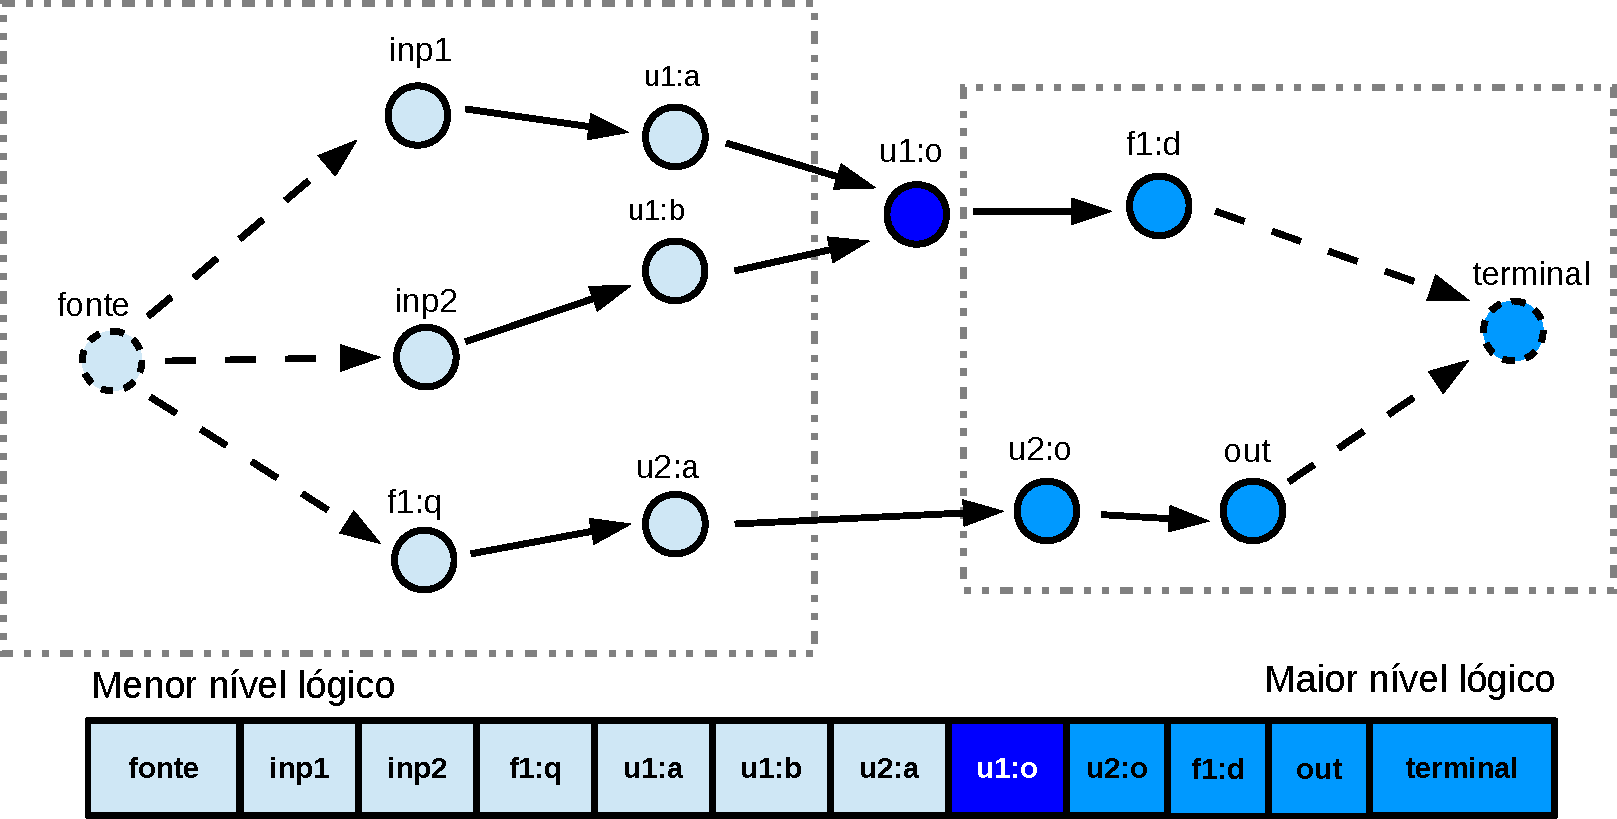
\includegraphics[width=\linewidth]{img/grafo_lista_nivel_logico.pdf} 
\caption{Na lista ordenada, observando o elemento \textit{u1:o}, os elementos de menor ou de igual  nível lógico (\textit{fonte, inp1, inp2, f1:q, u1:a, u1:b, u2:a}) se encontram à esquerda, e os de maior ou igual (\textit{u2:o, f1:d, out, terminal}) se encontram à direita.}
\label{fig:grafo_lista_nivel_logico}
\end{center}
\end{figure}

O algoritmo de STA é baseado nas técnicas conhecidas como PERT/CPM \cite{BhaskerChadha09}. Para melhorar o desempenho da técnica, foram adotadas estruturas de dados mais otimizadas para armazenar o grafo: ao guardar os dados do grafo em listas ordenadas topologicamente (Figura \ref{fig:grafo_lista_nivel_logico}), o algoritmo passa a ser apenas uma varredura em cada item da lista, atualizando as informações temporais previamente calculadas. Assim, não é mais necessário o uso da fila da técnica PERT/CPM.

\subsection{O Trabalho de Conclusão de Curso Gerado}
\label{sec:tcc}
O trabalho desenvolvido gerou a monografia de conclusão de curso intitulada ``Análise de \textit{Timing} Estática e a Avaliação do Impacto do Atraso das Interconexões em Circuitos Digitais'' e apresentada em Novembro de 2013. A mesma pode ser acessada no \textit{site} de projetos do curso de Ciências da Computação da UFSC \cite{linkTCC}.


\subsection{Validação e Resultados}

Para realizar a avaliação das técnicas abordadas neste trabalho, uma ferramenta para análise de \textit{timing} na linguagem de programação C++ foi implementada. A ferramenta realiza a análise de \textit{timing} e considera dois possíveis modelos de interconexão: o modelo da capacitância concentrada e o modelo RC concentrado.

Como parte dos experimentos é realizada comparando as informações calculadas pela ferramenta implementada com as informações reportadas pelo \textit{PrimeTime}, o erro percentual ($EP_t$) e o erro médio percentual absoluto ($EMPA$) (Equações \ref{eq:ep} e \ref{eq:empa}) foram adotados como métricas para estimar a qualidade das informações de \textit{timing} reportadas pela ferramenta implementada neste trabalho.

\begin{equation}
\label{eq:ep}
EP_t = \frac{(A_t - P_t)}{A_t} \times 100
\end{equation}

\begin{equation}
\label{eq:empa}
EMPA = \frac{\sum_{t=1}^n |EP_t|}{n}
\end{equation}

O erro percentual é calculado para cada uma das informações comparadas com o \textit{PrimeTime} utilizando a equação \ref{eq:ep}, sendo que $A_t$ é a informação obtida pelo \textit{PrimeTime} e $P_t$ é a informação calculada pela ferramenta implementada. Tais informações usadas para fim de validação da ferramenta foram:

\begin{itemize}
\item \textbf{\textit{TNS (Total Negative Slack)}: } O somatório de \textit{slack} negativo nas saídas primárias.

\item \textbf{\textit{Violating POs: }} Número de saídas primárias violando a restrição de desempenho mínimo.

\item \textbf{\textit{Runtime (s): }} Tempo de execução, em segundos, para realizar uma análise de \textit{timing} em um circuito, desconsiderando o tempo constante de inicialização da ferramenta.

\item \textbf{\textit{Critical Path: }} Valor do caminho crítico do circuito.
\end{itemize}

Os resultados dos experimentos serão apresentados posteriormente por meio de gráficos, tabelas e histogramas.

Este trabalho utilizou como base a infraestrutura disponibilizada pela competição de \textit{gate sizing} discreto do ISPD de 2013, a qual fornece:

\begin{itemize}

\item Um conjunto de 8 circuitos da competição do ISPD de 2013:
	\begin{enumerate}
	\item \textbf{$usb\_phy$}: com 511 células combinacionais, 98 células sequenciais, 15 entradas e 19 saídas primárias;
	\item \textbf{$pci\_bridge32$}: com 27316 células combinacionais, 3359 células sequenciais, 160 entradas e 201 saídas primárias;
	\item \textbf{$fft$}: com 30297 células combinacionais, 1984 células sequenciais, 1026 entradas e 1026 saídas primárias;
	\item \textbf{$cordic$}: com 40371 células combinacionais, 1230 células sequenciais, 34 entradas e 64 saídas primárias;
	\item \textbf{$des\_perf$}: com 103842 células combinacionais, 8802 células sequenciais, 234 entradas e 201 saídas primárias;
	\item \textbf{$edit\_dist$}: com 125000 células combinacionais, 5661 células sequenciais, 2562 entradas e 12 saídas primárias;
	\item \textbf{$matrix\_mult$}: com 30297 células combinacionais, 1984 células sequenciais, 3202 entradas e 1600 saídas primárias;
	\item \textbf{$netcard$}: com 884427 células combinacionais, 97831 células sequenciais, 1836 entradas e 10 saídas primárias.
	\end{enumerate}

\item Uma biblioteca \textit{standard cell} realista, composta por onze células combinacionais de diversas funções lógicas e um célula sequencial;

\item Uma ferramenta de análise de \textit{timing} estática PrimeTime \texttrademark \ da empresa \citeonline{PrimeTime12} \textregistered \ para comparação de resultados;
\end{itemize}

Os circuitos são compostos por descrições no formato Verilog, capacitâncias parasitas e resistências descritas no formato IEEE SPEF (\textit{Standard Parasitic Exchange Format}) \cite{IEEE99}, e restrições de \textit{timing} descritas no formato SDC (\textit{Synopsys Design Constraints}).

Os resultados dos experimentos realizados para validar a ferramenta de STA desenvolvida mostram alguns aspectos importantes:

\begin{itemize}
	\item A desconsideração da degradação do \textit{slew} na análise de \textit{timing} pode acarretar erros de cerca de 20\%;
	\item A técnica para cálculo das informações temporais das interconexões implementada apresentou ser \textbf{17,02 vezes mais rápida} que o PrimeTime, obtendo resultados para \textit{TNS (Total Negative Slack)} e \textit{critical path} que subestimam em cerca de 8,85\% e 4,48\% respectivamente, os reportados pela ferramenta industrial;
	\item A relação $C{eff} / C_{total}$ nos circuitos da competição de \textit{sizing} do ISPD de 2013 mostrou-se na média, próxima de 1. A partir dessa informação, o modelo de capacitância concentrada para calcular os atrasos dos \textit{drivers}, juntamente com a técnica de Elmore com $C_{total}$ e a técnica de \citeonline{PURI02} para degradação do \textit{slew} foi avaliada, apresentando estimativas pessimistas em 10,76\% para \textit{TNS} nos circuitos testados (exceto o $netcard$) e 6,48\% para \textit{critical path}, sendo que o tempo de execução é cerca de \textbf{3 vezes menor} que o da técnica considerando a $C_{eff}$. 
\end{itemize}

% ---
% Finaliza a parte no bookmark do PDF
% para que se inicie o bookmark na raiz
% e adiciona espaço de parte no Sumário
% ---
\phantompart

% ---
% Conclusão
% ---
\chapter*[Considerações finais]{Considerações finais}
\addcontentsline{toc}{chapter}{Considerações finais}

Durante o período de vigência da bolsa, o bolsista avaliou uma técnica de análise de \textit{timing} estática que considera os atrasos das interconexões e os efeito de degradação do \textit{slew} através destas. Para tal, o bolsista implementou uma ferramenta baseada na infraestrutura do ISPD de 2013 \cite{Contest2013} com os algoritmos para cálculos dos atrasos devidamente implementados. No fim da vigência da bolsa, foi também iniciada a incorporação do modelo de grafo e cálculos de atraso em uma técnica de otimização para fluxo industrial, conhecida como \textit{gate sizing}, porém com término previsto para metade do primeiro semestre de 2014.



% ----------------------------------------------------------
% ELEMENTOS PÓS-TEXTUAIS
% ----------------------------------------------------------
\postextual

% ----------------------------------------------------------
% Referências bibliográficas
% ----------------------------------------------------------
\bibliography{bolsa20132014}


\end{document}
